

\tikzset{every picture/.style={line width=0.75pt}} %set default line width to 0.75pt        

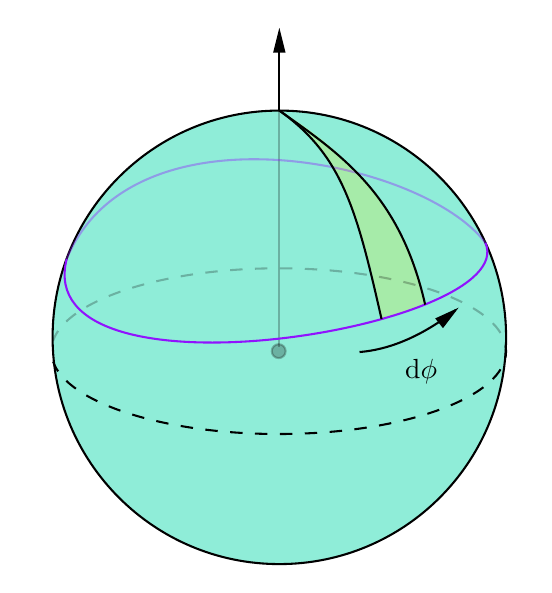
\begin{tikzpicture}[x=0.75pt,y=0.75pt,yscale=-1,xscale=1]
%uncomment if require: \path (0,300); %set diagram left start at 0, and has height of 300

%Shape: Circle [id:dp5046650378220048] 
\draw  [fill={rgb, 255:red, 80; green, 227; blue, 194 }  ,fill opacity=0.64 ] (262.21,175.75) .. controls (262.21,115.41) and (311.12,66.5) .. (371.46,66.5) .. controls (431.79,66.5) and (480.71,115.41) .. (480.71,175.75) .. controls (480.71,236.09) and (431.79,285) .. (371.46,285) .. controls (311.12,285) and (262.21,236.09) .. (262.21,175.75) -- cycle ;
%Shape: Polygon Curved [id:ds5250467240215824] 
\draw  [draw opacity=0][fill={rgb, 255:red, 184; green, 233; blue, 134 }  ,fill opacity=0.57 ] (371.46,66.5) .. controls (394.94,79.85) and (433.74,111.85) .. (441.71,159.98) .. controls (438.71,161.98) and (432.94,163.05) .. (420.71,166.98) .. controls (416.54,145.45) and (406.14,87.05) .. (371.46,66.5) -- cycle ;
%Shape: Arc [id:dp639258111017756] 
\draw  [draw opacity=0][dash pattern={on 4.5pt off 4.5pt}] (480.45,185.11) .. controls (480.62,184.23) and (480.7,183.33) .. (480.7,182.42) .. controls (480.7,160.38) and (431.66,142.5) .. (371.16,142.49) .. controls (315.32,142.48) and (269.23,157.69) .. (262.46,177.37) -- (371.15,182.41) -- cycle ; \draw  [color={rgb, 255:red, 0; green, 0; blue, 0 }  ,draw opacity=0.25 ][dash pattern={on 4.5pt off 4.5pt}] (480.45,185.11) .. controls (480.62,184.23) and (480.7,183.33) .. (480.7,182.42) .. controls (480.7,160.38) and (431.66,142.5) .. (371.16,142.49) .. controls (315.32,142.48) and (269.23,157.69) .. (262.46,177.37) ;
%Straight Lines [id:da9099277732366831] 
\draw    (371.46,28.61) -- (371.46,66.5) ;
\draw [shift={(371.46,26.61)}, rotate = 90] [fill={rgb, 255:red, 0; green, 0; blue, 0 }  ][line width=0.08]  [draw opacity=0] (12,-3) -- (0,0) -- (12,3) -- cycle    ;
%Straight Lines [id:da5824346930589386] 
\draw [color={rgb, 255:red, 0; green, 0; blue, 0 }  ,draw opacity=0.25 ]   (371.46,66.5) -- (371.46,180.53) ;
%Shape: Arc [id:dp687936282701906] 
\draw  [draw opacity=0][dash pattern={on 4.5pt off 4.5pt}] (480.45,179.7) .. controls (480.62,180.58) and (480.7,181.48) .. (480.7,182.39) .. controls (480.7,204.43) and (431.66,222.31) .. (371.16,222.33) .. controls (315.32,222.34) and (269.23,207.12) .. (262.46,187.44) -- (371.15,182.41) -- cycle ; \draw  [dash pattern={on 4.5pt off 4.5pt}] (480.45,179.7) .. controls (480.62,180.58) and (480.7,181.48) .. (480.7,182.39) .. controls (480.7,204.43) and (431.66,222.31) .. (371.16,222.33) .. controls (315.32,222.34) and (269.23,207.12) .. (262.46,187.44) ;
%Straight Lines [id:da1722555323787216] 
\draw    (262,168.95) ;
%Straight Lines [id:da03626750387054689] 
\draw [color={rgb, 255:red, 0; green, 0; blue, 0 }  ,draw opacity=0.25 ]   (371.15,182.41) ;
\draw [shift={(371.15,182.41)}, rotate = 0] [color={rgb, 255:red, 0; green, 0; blue, 0 }  ,draw opacity=0.25 ][fill={rgb, 255:red, 0; green, 0; blue, 0 }  ,fill opacity=0.25 ][line width=0.75]      (0, 0) circle [x radius= 3.35, y radius= 3.35]   ;
%Curve Lines [id:da11755103924593024] 
\draw [color={rgb, 255:red, 144; green, 19; blue, 254 }  ,draw opacity=1 ]   (269,138) .. controls (250.71,210.2) and (488.71,171.2) .. (470.71,130.2) ;
%Curve Lines [id:da05946487398733602] 
\draw [color={rgb, 255:red, 144; green, 19; blue, 254 }  ,draw opacity=0.37 ]   (269,138) .. controls (300.71,61.2) and (440.71,90.2) .. (470.71,130.2) ;
%Curve Lines [id:da02604208213784487] 
\draw    (371.46,66.5) .. controls (401.71,87.98) and (408.71,113.98) .. (420.71,166.98) ;
%Curve Lines [id:da2819669603292758] 
\draw    (371.46,66.5) .. controls (401.71,87.98) and (429.71,106.98) .. (441.71,159.98) ;
%Curve Lines [id:da37610290595360074] 
\draw    (410.1,182.83) .. controls (429.9,181.25) and (446.72,170.14) .. (456.34,162.64) ;
\draw [shift={(457.8,161.48)}, rotate = 501.33] [fill={rgb, 255:red, 0; green, 0; blue, 0 }  ][line width=0.08]  [draw opacity=0] (12,-3) -- (0,0) -- (12,3) -- cycle    ;

% Text Node
\draw (439.79,184.69) node [anchor=north] [inner sep=0.75pt]    {$\mathrm{d} \phi $};


\end{tikzpicture}
